% Source: pca_through_affine_spaces.tex
\begin{notechapter}
\chapter{PCA through Affine Spaces}\label{ch:pca-affine}
\chaptersubtitle{A geometric foundation}

\section{Introduction}

Principal Component Analysis (PCA) is typically presented as an eigenvector computation or matrix factorization technique. However, its geometric essence becomes clearer when viewed through the lens of \textbf{affine spaces}. This perspective naturally separates the \textbf{point-like} nature of data from the \textbf{vector-like} operations we perform, providing deeper insight into why PCA works and what it truly accomplishes geometrically.

\section{Affine Spaces: A Brief Review}

\begin{definition}
An \textbf{affine space} is a triple $(A, V, +)$ where:
\begin{itemize}
    \item $A$ is a set (the ``points'')
    \item $V$ is a vector space (the ``direction space'' or ``translation space'')
    \item $+ : A \times V \to A$ is a map satisfying:
    \begin{enumerate}
        \item For every $p \in A$ and $v,w \in V$: $(p + v) + w = p + (v + w)$
        \item For every $p,q \in A$, there exists a unique $v \in V$ such that $p + v = q$
    \end{enumerate}
\end{itemize}
\end{definition}

In our context, we take $A = \mathbb{R}^n$ and $V = \mathbb{R}^n$ with the natural action.

\begin{remark}
The key distinction: \textbf{points} (elements of $A$) have positions but no inherent direction, while \textbf{vectors} (elements of $V$) represent displacements and can be applied to any point. This separation clarifies that data points exist in space, while principal components are directions in that space.
\end{remark}

\section{Data as Points in Affine Space}

Consider a dataset with $m$ samples and $n$ features, represented as a matrix:
\[
X = \begin{bmatrix}
x_{11} & \cdots & x_{1n} \\
\vdots & \ddots & \vdots \\
x_{m1} & \cdots & x_{mn}
\end{bmatrix}
\]

We interpret this data in the \textbf{feature space perspective}:

\subsection{Feature Space Perspective ($\mathbb{R}^n$)}
Each \textbf{row} $x_i = (x_{i1}, \dots, x_{in})$ represents a point in the affine space $A = \mathbb{R}^n$. Here, $n$ is the number of features. The points are samples, and the space is defined by the features.

\begin{remark}
This is the standard view for PCA: we have $m$ data points living in an $n$-dimensional feature space. Our goal is to find low-dimensional affine subspaces that approximate these points well.
\end{remark}

\section{The Centering Operation: Moving to Barycentric Coordinates}

\subsection{Centering in Feature Space}

Define the \textbf{centroid of the data} (vector of feature means):
\[
\bar{x} = \frac{1}{m}\sum_{i=1}^m x_i \in A
\]

\begin{remark}[Interpretation of $\bar{x}$]
The point $\bar{x}$ represents the \textbf{prototypical sample} or \textbf{average data point}. Each coordinate $j$ of $\bar{x}$ is the average value of feature $j$ across all $m$ samples. Geometrically, $\bar{x}$ is the centroid of all data points in the feature space $\mathbb{R}^n$.
\end{remark}

The \textbf{centered data} are displacement vectors:
\[
x_i' = x_i - \bar{x} \in V
\]
These represent positions relative to the data centroid.

\subsection{Matrix Formulation of Centering}

Define the centering matrix:
\[
C_m = I_m - \frac{1}{m}\mathbf{1}_m\mathbf{1}_m^T
\]
where $\mathbf{1}_m$ is the $m$-dimensional vector of ones.

The centered data matrix is:
\[
X_{\text{centered}} = C_m X
\]

\begin{figure}[h]
\centering
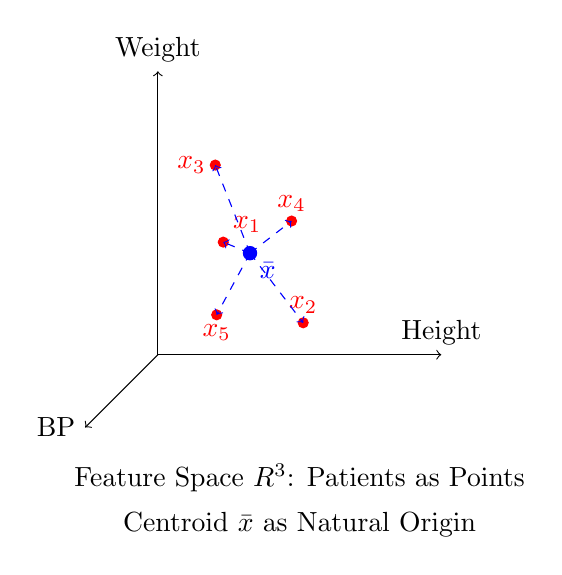
\begin{tikzpicture}[scale=1.2]
    % Axes
    \draw[->] (0,0,0) -- (3,0,0) node[above] {Height};
    \draw[->] (0,0,0) -- (0,3,0) node[above] {Weight};
    \draw[->] (0,0,0) -- (0,0,2) node[left] {BP};
    
    % Data points (patients)
    \filldraw[red] (1,1.5,0.8) circle (1.5pt) node[above right] {$x_1$};
    \filldraw[red] (2,0.8,1.2) circle (1.5pt) node[above] {$x_2$};
    \filldraw[red] (0.8,2.2,0.5) circle (1.5pt) node[left] {$x_3$};
    \filldraw[red] (1.8,1.8,1.0) circle (1.5pt) node[above] {$x_4$};
    \filldraw[red] (1.2,1.0,1.5) circle (1.5pt) node[below] {$x_5$};
    
    % Mean point
    \filldraw[blue] (1.36,1.46,1.0) circle (2pt) node[below right] {$\bar{x}$};
    
    % Displacement vectors
    \draw[blue,->,dashed] (1.36,1.46,1.0) -- (1,1.5,0.8);
    \draw[blue,->,dashed] (1.36,1.46,1.0) -- (2,0.8,1.2);
    \draw[blue,->,dashed] (1.36,1.46,1.0) -- (0.8,2.2,0.5);
    \draw[blue,->,dashed] (1.36,1.46,1.0) -- (1.8,1.8,1.0);
    \draw[blue,->,dashed] (1.36,1.46,1.0) -- (1.2,1.0,1.5);
    
    % Title
    \node at (1.5,-1.3) {Feature Space $\mathbb{R}^3$: Patients as Points};
    \node at (1.5,-1.8) {Centroid $\bar{x}$ as Natural Origin};
\end{tikzpicture}
\caption{Feature space representation: data points in $\mathbb{R}^3$ with features as axes. Centering moves the origin to the data centroid $\bar{x}$.}
\end{figure}

\subsection*{Example: Centering a Small Dataset}

Consider a simple dataset with $m = 2$ patients and $n = 3$ features:

\[
X = \begin{bmatrix}
\text{Height} & \text{Weight} & \text{BP} \\
170 & 70 & 120 \\  % Patient 1
180 & 65 & 140     % Patient 2
\end{bmatrix}
\]

First, compute the matrix of means by applying the averaging operation:

\[
\frac{1}{2}\mathbf{1}_2\mathbf{1}_2^T X = \frac{1}{2}
\begin{bmatrix}
1 & 1 \\
1 & 1
\end{bmatrix}
\begin{bmatrix}
170 & 70 & 120 \\
180 & 65 & 140
\end{bmatrix}
= \frac{1}{2}
\begin{bmatrix}
350 & 135 & 260 \\
350 & 135 & 260
\end{bmatrix}
= 
\begin{bmatrix}
175 & 67.5 & 130 \\
175 & 67.5 & 130
\end{bmatrix}
\]

Each row of this matrix is the mean vector $\bar{x} = (175, 67.5, 130)$.

Now compute the centered data by subtracting the means:

\[
X_{\text{centered}} = X - \frac{1}{2}\mathbf{1}_2\mathbf{1}_2^T X = 
\begin{bmatrix}
170 & 70 & 120 \\
180 & 65 & 140
\end{bmatrix}
- 
\begin{bmatrix}
175 & 67.5 & 130 \\
175 & 67.5 & 130
\end{bmatrix}
= 
\begin{bmatrix}
-5 & 2.5 & -10 \\
5 & -2.5 & 10
\end{bmatrix}
\]

\begin{remark}[Interpretation of the Result]
The centered matrix shows each patient's deviation from the average:
\begin{itemize}
    \item Patient 1: 5cm shorter, 2.5kg heavier, 10mmHg lower BP than average
    \item Patient 2: 5cm taller, 2.5kg lighter, 10mmHg higher BP than average  
    \item The centroid is $\bar{x} = (175, 67.5, 130)$
    \item Each column sums to zero, confirming proper centering
\end{itemize}
The displacement vectors $x_1' = (-5, 2.5, -10)$ and $x_2' = (5, -2.5, 10)$ represent positions relative to the centroid in the 3D feature space.
\end{remark}

\section{The Covariance Structure in Feature Space}

\subsection{Feature Covariance Matrix}

\begin{definition}[Feature Covariance Matrix]
Given the feature-centered data matrix $X_{\text{centered}}$ where each feature has mean zero:
\[
\frac{1}{m}\sum_{i=1}^m x_{ij} = 0 \quad \text{for all } j = 1,\dots,n
\]
the feature covariance matrix is:
\[
S_{\text{features}} = \frac{1}{m}X_{\text{centered}}^T X_{\text{centered}}
\]
with entries:
\[
(S_{\text{features}})_{jk} = \frac{1}{m}\sum_{i=1}^m (x_{ij} - \bar{x}_j)(x_{ik} - \bar{x}_k) = \frac{1}{m}\sum_{i=1}^m x_{ij}x_{ik}
\]
\end{definition}

\begin{proof}
Since $\bar{x}_j = \frac{1}{m}\sum_{i=1}^m x_{ij}$ and $\bar{x}_k = \frac{1}{m}\sum_{i=1}^m x_{ik}$, we have:
\begin{align*}
(S_{\text{features}})_{jk} &= \frac{1}{m}\sum_{i=1}^m (x_{ij} - \bar{x}_j)(x_{ik} - \bar{x}_k) \\
&= \Big(\frac{1}{m}\sum_{i=1}^m x_{ij}x_{ik}\Big) - \bar{x}_j\bar{x}_k - \bar{x}_j\bar{x}_k + \bar{x}_j\bar{x}_k \\
&= \Big(\frac{1}{m}\sum_{i=1}^m x_{ij}x_{ik}\Big) - \bar{x}_j\bar{x}_k
\end{align*}
But since $\bar{x}_j = \frac{1}{m}\sum_{i=1}^m x_{ij} = 0$ and $\bar{x}_k = \frac{1}{m}\sum_{i=1}^m x_{ik} = 0$ for the centered data, we get:
\[
(S_{\text{features}})_{jk} = \frac{1}{m}\sum_{i=1}^m x_{ij}x_{ik}
\]
\end{proof}

\begin{remark}[Inner Product Interpretation]
We can express the feature covariance matrix in terms of the feature vectors $f_j \in \mathbb{R}^m$ (columns of $X_{\text{centered}}$). Let:
\[
F = X_{\text{centered}}^T = \begin{bmatrix}
\mid & \mid & & \mid \\
f_1 & f_2 & \cdots & f_n \\
\mid & \mid & & \mid
\end{bmatrix}
\]
Then the feature covariance matrix becomes:
\[
S_{\text{features}} = \frac{1}{m}FF^T = \frac{1}{m}
\begin{bmatrix}
\langle f_1, f_1 \rangle & \langle f_1, f_2 \rangle & \cdots & \langle f_1, f_n \rangle \\
\langle f_2, f_1 \rangle & \langle f_2, f_2 \rangle & \cdots & \langle f_2, f_n \rangle \\
\vdots & \vdots & \ddots & \vdots \\
\langle f_n, f_1 \rangle & \langle f_n, f_2 \rangle & \cdots & \langle f_n, f_n \rangle
\end{bmatrix}
\]

Each entry $(S_{\text{features}})_{jk} = \frac{1}{m}\langle f_j, f_k \rangle$ represents the scaled inner product between feature vectors $f_j$ and $f_k$.
\end{remark}

\begin{remark}[Geometric Interpretation]
This formulation reveals that:
\begin{itemize}
    \item \textbf{Diagonal entries}: $(S_{\text{features}})_{jj} = \frac{1}{m}\|f_j\|^2$ represent the variance of feature $j$
    \item \textbf{Off-diagonal entries}: $(S_{\text{features}})_{jk} = \frac{1}{m}\|f_j\|\|f_k\|\cos\theta_{jk}$ represent the covariance between features $j$ and $k$
    \item The matrix $S_{\text{features}}$ captures both the magnitudes and relative orientations of the feature vectors in sample space $\mathbb{R}^m$
\end{itemize}
\end{remark}

\begin{remark}[Population vs. Sample Covariance]
The matrix $S_{\text{features}}$ is a \textbf{sample covariance matrix} that estimates the population covariance. If we view our data as $m$ independent realizations of a random vector $\mathbf{X} = (X_1, \dots, X_n)$ with population covariance matrix $\Sigma$, then:

\[
S_{\text{features}} = \frac{1}{m}\sum_{i=1}^m (x_i - \bar{x})(x_i - \bar{x})^T
\]

is an estimator of $\Sigma = \mathbb{E}[(\mathbf{X} - \mu)(\mathbf{X} - \mu)^T]$, where $\mu = \mathbb{E}[\mathbf{X}]$.

\begin{itemize}
    \item The $(j,k)$ entry $(S_{\text{features}})_{jk}$ estimates $\text{Cov}(X_j, X_k)$
    \item The diagonal entries $(S_{\text{features}})_{jj}$ estimate $\text{Var}(X_j)$
    \item Using divisor $m$ (rather than $m-1$) gives the maximum likelihood estimator under Gaussian assumptions
\end{itemize}

In the geometric perspective, we treat $S_{\text{features}}$ as describing the empirical covariance structure of our specific dataset, while recognizing it as an estimate of the underlying population structure.
\end{remark}

\begin{remark}[Unbiased Version]
Some texts use the unbiased estimator:
\[
S_{\text{unbiased}} = \frac{1}{m-1}X_{\text{centered}}^T X_{\text{centered}}
\]
which differs from our definition by a factor of $\frac{m}{m-1}$. For PCA, this scaling factor affects the eigenvalues but not the eigenvectors (principal directions), so the geometric interpretation remains unchanged.
\end{remark}

\section{The Dual Perspective: Sample Space and Gram Matrix}

\subsection{Sample Space View}

Consider the columns of $X_{\text{centered}}$ as vectors in $\mathbb{R}^m$:
\[
f_j = (x_{1j}, x_{2j}, \dots, x_{mj}) \in \mathbb{R}^m
\]

\begin{figure}[h]
\centering
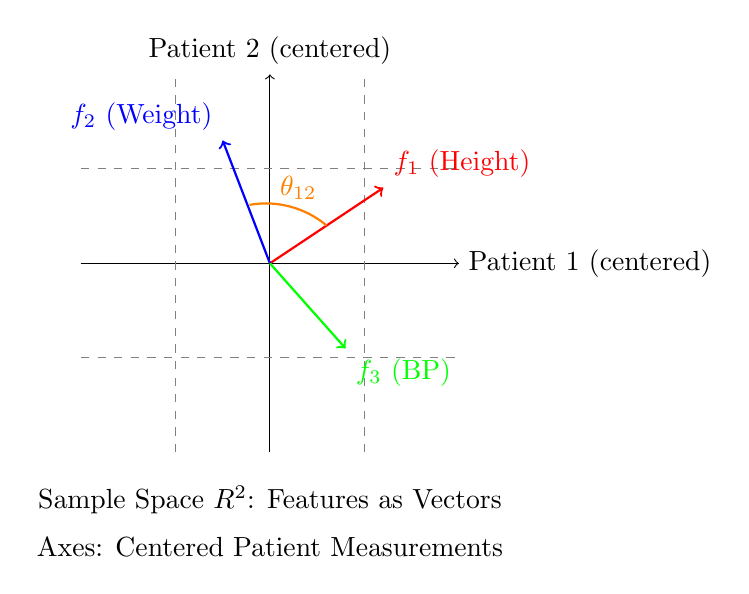
\begin{tikzpicture}[scale=1.2]
    % Axes
    \draw[->] (-2,0) -- (2,0) node[right] {Patient 1 (centered)};
    \draw[->] (0,-2) -- (0,2) node[above] {Patient 2 (centered)};
    
    % Coordinate lines
    \draw[gray, dashed] (1,-2) -- (1,2);
    \draw[gray, dashed] (-1,-2) -- (-1,2);
    \draw[gray, dashed] (-2,1) -- (2,1);
    \draw[gray, dashed] (-2,-1) -- (2,-1);
    
    % Feature vectors (from centered data)
    \draw[->,thick,red] (0,0) -- (1.2,0.8) node[above right] {$f_1$ (Height)};
    \draw[->,thick,blue] (0,0) -- (-0.5,1.3) node[above left] {$f_2$ (Weight)};
    \draw[->,thick,green] (0,0) -- (0.8,-0.9) node[below right] {$f_3$ (BP)};
    
    % Angle between red and blue vectors
    \draw[orange,thick] (0.6,0.4) arc (50:100:1);
    \node[orange] at (0.3,0.8) {$\theta_{12}$};
    
    % Title
    \node at (0,-2.5) {Sample Space $\mathbb{R}^2$: Features as Vectors};
    \node at (0,-3) {Axes: Centered Patient Measurements};
\end{tikzpicture}
\caption{Sample space representation: each feature is a vector in $\mathbb{R}^m$. The coordinates show how that feature varies across different patients. The angle $\theta$ between vectors indicates correlation between features.}
\end{figure}

\begin{remark}[Interpretation of Sample Space]
In this visualization:
\begin{itemize}
    \item Each axis represents a \textbf{patient} with centered measurements
    \item Each vector represents a \textbf{feature} showing its variation across patients
    \item Vector length indicates how much that feature varies across patients
    \item Angles between vectors indicate correlations between features
    \item The origin represents the average patient profile
\end{itemize}

For example, if height and weight vectors point in similar directions, they are positively correlated across patients.
\end{remark}

\begin{theorem}[Gram Matrix and Sample Covariance]
The Gram matrix $G = X_{\text{centered}} X_{\text{centered}}^T$ is related to a sample covariance matrix:

If we were to compute the covariance between samples (rather than features), we would need to center the data in sample space:
\[
X_{\text{doubly-centered}} = C_m X C_n
\]
Then the sample covariance matrix would be:
\[
S_{\text{samples}} = \frac{1}{n}X_{\text{doubly-centered}} X_{\text{doubly-centered}}^T
\]
However, in standard PCA, we work with:
\[
G = X_{\text{centered}} X_{\text{centered}}^T
\]
which measures sample similarities using uncentered sample means.
\end{theorem}

\subsection{Gram Matrix and Its Interpretation}

The Gram matrix $G = X_{\text{centered}} X_{\text{centered}}^T$ has a clear geometric interpretation in sample space:

\[
G = \begin{bmatrix}
\langle x_1', x_1' \rangle & \langle x_1', x_2' \rangle & \cdots & \langle x_1', x_m' \rangle \\
\langle x_2', x_1' \rangle & \langle x_2', x_2' \rangle & \cdots & \langle x_2', x_m' \rangle \\
\vdots & \vdots & \ddots & \vdots \\
\langle x_m', x_1' \rangle & \langle x_m', x_2' \rangle & \cdots & \langle x_m', x_m' \rangle
\end{bmatrix}
\]

where $x_i' = x_i - \bar{x}$ are the centered data points (rows of $X_{\text{centered}}$), and each entry $G_{ij} = \langle x_i', x_j' \rangle$ represents the dot product between the centered data points $x_i'$ and $x_j'$.

\begin{remark}[Geometric Meaning of Gram Matrix Entries]
\begin{itemize}
    \item []
    \item \textbf{Diagonal entries}: $G_{ii} = \|x_i'\|^2$ represent squared distances from the centroid
    \item \textbf{Off-diagonal entries}: $G_{ij} = \|x_i'\|\|x_j'\|\cos\theta_{ij}$ measure similarity between samples
    \item When $G_{ij} > 0$: samples $i$ and $j$ are on the same side of the centroid (acute angle between their displacement vectors)
    \item When $G_{ij} < 0$: samples $i$ and $j$ are on opposite sides of the centroid (obtuse angle between their displacement vectors)
    \item When $G_{ij} = 0$: samples $i$ and $j$ are orthogonal relative to the centroid
\end{itemize}
\end{remark}

\subsection{Connecting Feature Space and Sample Space}

The two perspectives are mathematically dual through the following relationships:

\begin{theorem}[Duality Between Feature Space and Sample Space]
For the centered data matrix $X_{\text{centered}} \in \mathbb{R}^{m \times n}$ with $m$ samples and $n$ features:

\begin{enumerate}
    \item \textbf{Feature Space Analysis}: The feature covariance matrix 
    \[
    S_{\text{features}} = \frac{1}{m}X_{\text{centered}}^T X_{\text{centered}} \in \mathbb{R}^{n \times n}
    \]
    captures covariances between features. Its eigenvectors are the principal directions in feature space $\mathbb{R}^n$.

    \item \textbf{Sample Space Analysis}: The Gram matrix
    \[
    G = X_{\text{centered}} X_{\text{centered}}^T \in \mathbb{R}^{m \times m}
    \]
    captures similarities between samples. Its eigenvectors represent dominant patterns across samples.

    \item \textbf{Spectral Connection}: The non-zero eigenvalues of $S_{\text{features}}$ and $\frac{1}{m}G$ are identical. Specifically, if $\lambda$ is a non-zero eigenvalue of $S_{\text{features}}$, then $m\lambda$ is an eigenvalue of $G$.

    \item \textbf{Eigenvector Mapping}: If $v \in \mathbb{R}^n$ is an eigenvector of $S_{\text{features}}$ with eigenvalue $\lambda > 0$, then $X_{\text{centered}}v \in \mathbb{R}^m$ is an eigenvector of $G$ with eigenvalue $m\lambda$.
\end{enumerate}
\end{theorem}

\begin{proof}
Let $X_{\text{centered}} = U\Sigma V^T$ be the singular value decomposition, where $U \in \mathbb{R}^{m \times r}$, $\Sigma \in \mathbb{R}^{r \times r}$, $V \in \mathbb{R}^{n \times r}$, and $r = \text{rank}(X_{\text{centered}})$.

\begin{enumerate}
    \item The feature covariance matrix decomposes as:
    \[
    S_{\text{features}} = \frac{1}{m}V\Sigma^2 V^T
    \]
    So $V$ contains the eigenvectors of $S_{\text{features}}$ with eigenvalues $\frac{1}{m}\sigma_i^2$.

    \item The Gram matrix decomposes as:
    \[
    G = U\Sigma^2 U^T
    \]
    So $U$ contains the eigenvectors of $G$ with eigenvalues $\sigma_i^2$.

    \item Both matrices share the squared singular values $\sigma_i^2$, scaled differently.

    \item For any eigenvector $v_j$ of $S_{\text{features}}$:
    \begin{align*}
    G(X_{\text{centered}}v_j) &= X_{\text{centered}}X_{\text{centered}}^T(X_{\text{centered}}v_j) \\
    &= X_{\text{centered}}(X_{\text{centered}}^T X_{\text{centered}}v_j) \\
    &= X_{\text{centered}}(m\lambda_j v_j) = m\lambda_j (X_{\text{centered}}v_j)
    \end{align*}
    Thus $X_{\text{centered}}v_j$ is an eigenvector of $G$ with eigenvalue $m\lambda_j$.
\end{enumerate}
\end{proof}

\begin{remark}[Practical Interpretation of the Duality]
The duality allows us to:
\begin{itemize}
    \item \textbf{Compute PCA in either space}: For datasets with $m \ll n$ (few samples, many features), it's computationally cheaper to work with $G$ ($m \times m$) rather than $S_{\text{features}}$ ($n \times n$)
    \item \textbf{Interpret results in both spaces}: Principal components in feature space correspond to directions of maximum variance, while in sample space they correspond to directions that best separate the samples
    \item \textbf{Understand kernel methods}: The Gram matrix is fundamental to kernel PCA, where we replace dot products with kernel functions
\end{itemize}
\end{remark}

\begin{remark}[Visualizing the Connection]
Using our earlier $2 \times 3$ example with centered data:
\[
X_{\text{centered}} = \begin{bmatrix}
-5 & 2.5 & -10 \\
5 & -2.5 & 10
\end{bmatrix}
\]

The feature covariance matrix ($3 \times 3$) captures relationships between features:
\[
S_{\text{features}} = \frac{1}{2}X_{\text{centered}}^T X_{\text{centered}}
\]

The Gram matrix ($2 \times 2$) captures relationships between samples:
\[
G = X_{\text{centered}} X_{\text{centered}}^T = \begin{bmatrix}
131.25 & -131.25 \\
-131.25 & 131.25
\end{bmatrix}
\]

The large negative off-diagonal entry in $G$ indicates that the two patients are very dissimilar (on opposite sides of the centroid across all features).
\end{remark}

\subsection{Complete Example: Visualizing the Duality}

Let's complete our $2 \times 3$ example to illustrate the duality between feature space and sample space PCA.

\subsubsection*{Feature Space PCA}

Our centered data:
\[
X_{\text{centered}} = \begin{bmatrix}
-5 & 2.5 & -10 \\
5 & -2.5 & 10
\end{bmatrix}
\]

Feature covariance matrix:
\[
S_{\text{features}} = \frac{1}{2}X_{\text{centered}}^T X_{\text{centered}} = \frac{1}{2}
\begin{bmatrix}
50 & -25 & 100 \\
-25 & 12.5 & -50 \\
100 & -50 & 200
\end{bmatrix}
= \begin{bmatrix}
25 & -12.5 & 50 \\
-12.5 & 6.25 & -25 \\
50 & -25 & 100
\end{bmatrix}
\]

Eigen decomposition of $S_{\text{features}}$:
\begin{itemize}
    \item Eigenvalues: $\lambda_1 = 131.25, \lambda_2 = 0, \lambda_3 = 0$
    \item Principal direction (eigenvector): $v_1 = \frac{1}{\sqrt{21}}(2, -1, 4)$
    \item The data lies entirely along this direction in feature space
\end{itemize}

\subsubsection*{Sample Space PCA}

Gram matrix:
\[
G = X_{\text{centered}} X_{\text{centered}}^T = \begin{bmatrix}
131.25 & -131.25 \\
-131.25 & 131.25
\end{bmatrix}
\]

Eigen decomposition of $G$:
\begin{itemize}
    \item Eigenvalues: $\mu_1 = 262.5, \mu_2 = 0$
    \item Principal direction (eigenvector): $u_1 = \frac{1}{\sqrt{2}}(1, -1)$
    \item Note: $\mu_1 = 2\lambda_1 = m\lambda_1$ as predicted by the duality theorem
\end{itemize}

\begin{figure}[h]
\centering
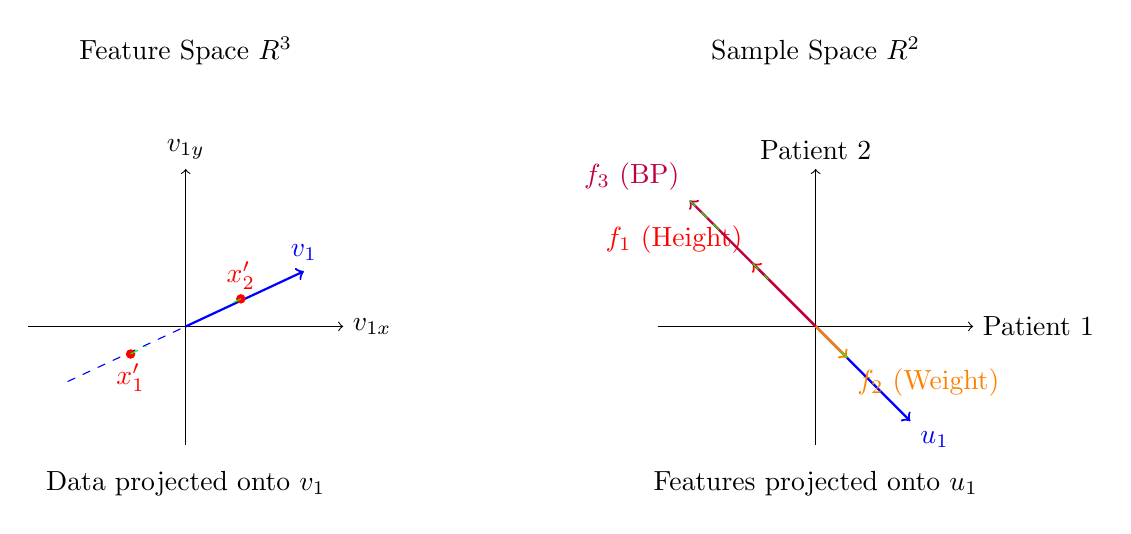
\begin{tikzpicture}
% Feature Space (left)
\begin{scope}[xshift=-4cm]
    \node at (0,3.5) {Feature Space $\mathbb{R}^3$};
    
    % Simplified 2D projection for visualization
    \draw[->] (-2,0) -- (2,0) node[right] {$v_{1x}$};
    \draw[->] (0,-1.5) -- (0,2) node[above] {$v_{1y}$};
    
    % Principal direction
    \draw[->, thick, blue] (0,0) -- (1.5,0.7) node[above] {$v_1$};
    \draw[blue, dashed] (-1.5,-0.7) -- (1.5,0.7);
    
    % Data points projected
    \filldraw[red] (-0.7,-0.35) circle (1.5pt) node[below] {$x_1'$};
    \filldraw[red] (0.7,0.35) circle (1.5pt) node[above] {$x_2'$};
    
    % Projections onto PC
    \draw[green, dashed] (-0.7,-0.35) -- (-0.5,-0.25);
    \draw[green, dashed] (0.7,0.35) -- (0.5,0.25);
    
    \node at (0,-2) {Data projected onto $v_1$};
\end{scope}

% Sample Space (right)
\begin{scope}[xshift=4cm]
    \node at (0,3.5) {Sample Space $\mathbb{R}^2$};
    
    % Axes
    \draw[->] (-2,0) -- (2,0) node[right] {Patient 1};
    \draw[->] (0,-1.5) -- (0,2) node[above] {Patient 2};
    
    % Principal direction
    \draw[->, thick, blue] (0,0) -- (1.2,-1.2) node[below right] {$u_1$};
    \draw[blue, dashed] (-1.2,1.2) -- (1.2,-1.2);
    
    % Feature vectors
    \draw[->, thick, red] (0,0) -- (-0.8,0.8) node[above left] {$f_1$ (Height)};
    \draw[->, thick, orange] (0,0) -- (0.4,-0.4) node[below right] {$f_2$ (Weight)};
    \draw[->, thick, purple] (0,0) -- (-1.6,1.6) node[above left] {$f_3$ (BP)};
    
    % Projections
    \draw[green, dashed] (-0.8,0.8) -- (-0.6,0.6);
    \draw[green, dashed] (0.4,-0.4) -- (0.3,-0.3);
    \draw[green, dashed] (-1.6,1.6) -- (-1.2,1.2);
    
    \node at (0,-2) {Features projected onto $u_1$};
\end{scope}
\end{tikzpicture}
\caption{Duality visualization: In feature space (left), samples project onto principal direction $v_1$. In sample space (right), features project onto principal direction $u_1$. The eigenvalue relationship $\mu_1 = m\lambda_1$ connects both spaces.}
\end{figure}

\begin{remark}[Interpretation of the Duality]
\begin{itemize}
    \item []
    \item \textbf{Feature Space}: The single principal direction $v_1 = (2,-1,4)/\sqrt{21}$ indicates that Height, Weight, and Blood Pressure vary together in fixed proportions (2:-1:4). The negative sign for Weight suggests it moves opposite to Height and BP in the dominant pattern.
    
    \item \textbf{Sample Space}: The principal direction $u_1 = (1,-1)/\sqrt{2}$ represents the dominant pattern of variation across patients. The coordinates $(1,-1)$ mean:
    \begin{itemize}
        \item When this pattern is \textbf{positive}, Patient 1 has above-average measurements and Patient 2 has below-average measurements
        \item When this pattern is \textbf{negative}, Patient 1 has below-average measurements and Patient 2 has above-average measurements
        \item The pattern captures the \textbf{contrast} between the two patients
    \end{itemize}
    
    \item \textbf{Connection}: $X_{\text{centered}}v_1$ is proportional to $u_1$, confirming the eigenvector mapping:
    \[
    X_{\text{centered}}v_1 = \begin{bmatrix}
    -5 & 2.5 & -10 \\
    5 & -2.5 & 10
    \end{bmatrix}
    \frac{1}{\sqrt{21}}\begin{bmatrix}2\\-1\\4\end{bmatrix}
        = \frac{1}{\sqrt{21}}\begin{bmatrix}-52.5\\52.5\end{bmatrix}
    \propto \begin{bmatrix}1\\-1\end{bmatrix} = \sqrt{2}u_1
    \]
    
    This shows that projecting the data onto the feature-space principal direction $v_1$ gives us exactly the sample-space principal direction $u_1$ (up to scaling and sign). As predicted by the SVD, $\|X_{\text{centered}}v_1\| = \frac{52.5\sqrt{2}}{\sqrt{21}} = \sqrt{262.5} = \sqrt{\mu_1}$, the singular value $\sigma_1$.
\end{itemize}
\end{remark}

\section{Standardization and Unit Vectors in Sample Space}

\subsection{Normalizing Feature Vectors to Unit Length}

\begin{theorem}[Unit Vector Condition]
A feature vector $f_j = (x_{1j}, x_{2j}, \dots, x_{mj})$ has unit length if and only if:
\[
\|f_j\|^2 = \sum_{i=1}^m x_{ij}^2 = 1
\]
For centered data where $\frac{1}{m}\sum_{i=1}^m x_{ij} = 0$, this is equivalent to the feature having variance $\frac{1}{m}$.
\end{theorem}

\subsection{Operation for Unit Vectors}

To transform all feature vectors to unit length, we apply \textbf{standardization}:

\begin{definition}[Feature Standardization]
Let $\sigma_j = \sqrt{\frac{1}{m}\sum_{i=1}^m (x_{ij} - \bar{x}_j)^2}$ be the sample standard deviation of feature $f_j$ (the $j$-th column of $X_{\text{centered}}$). The standardized data matrix is:
\[
X_{\text{standardized}} = X_{\text{centered}} D^{-1}
\]
where $D = \text{diag}(\sigma_1, \sigma_2, \dots, \sigma_n)$.
\end{definition}

\begin{remark}[Variance Interpretation]
Since $X_{\text{centered}}$ has zero-mean columns, the sample variance of feature $f_j$ is:
\[
s_j^2 = \frac{1}{m}\sum_{i=1}^m (x_{ij} - \bar{x}_j)^2 = \sigma_j^2
\]
Thus $\sigma_j$ is the sample standard deviation of feature $f_j$, and standardization transforms each feature to have unit sample variance:
\[
\frac{1}{m}\sum_{i=1}^m \left(\frac{x_{ij} - \bar{x}_j}{\sigma_j}\right)^2 = 1
\]
\end{remark}

\begin{remark}[Population vs. Sample Terminology]
\begin{itemize}
    \item[]
    \item $\sigma_j$ is a \textbf{sample statistic} that estimates the population standard deviation
    \item Using divisor $m$ gives the maximum likelihood estimator under Gaussian assumptions
    \item Some texts use $\frac{1}{m-1}$ for unbiased estimation, but this doesn't affect the geometric interpretation
    \item In the geometric perspective, we work with the empirical distribution of our specific dataset
\end{itemize}
\end{remark}

\begin{theorem}[Unit Vector Property]
The columns of $X_{\text{standardized}}$ have length $\sqrt{m}$:
\[
\|f_j^{\text{std}}\|^2 = \sum_{i=1}^m \left(\frac{x_{ij} - \bar{x}_j}{\sigma_j}\right)^2 = m
\]
and therefore the normalized vectors $\frac{1}{\sqrt{m}}f_j^{\text{std}}$ have unit length.
\end{theorem}

\begin{proof}
For standardized features:
\[
\sigma_j^2 = \frac{1}{m}\sum_{i=1}^m (x_{ij} - \bar{x}_j)^2
\]
So:
\[
\sum_{i=1}^m \left(\frac{x_{ij} - \bar{x}_j}{\sigma_j}\right)^2 = \frac{1}{\sigma_j^2}\sum_{i=1}^m (x_{ij} - \bar{x}_j)^2 = \frac{1}{\sigma_j^2}(m\sigma_j^2) = m
\]
Thus $\|\frac{1}{\sqrt{m}}f_j^{\text{std}}\| = 1$.
\end{proof}

\begin{figure}[h]
\centering
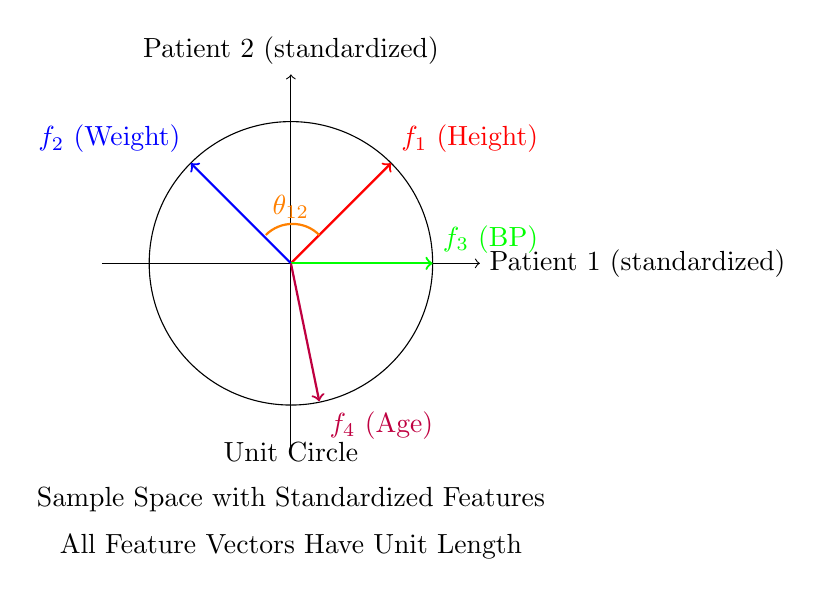
\begin{tikzpicture}[scale=1.2]
    % Unit circle
    \draw (0,0) circle (1.5cm);
    \node at (0,-2) {Unit Circle};
    
    % Axes
    \draw[->] (-2,0) -- (2,0) node[right] {Patient 1 (standardized)};
    \draw[->] (0,-2) -- (0,2) node[above] {Patient 2 (standardized)};
    
    % Unit vectors (all on circle)
    \draw[->,thick,red] (0,0) -- (1.06,1.06) node[above right] {$f_1$ (Height)};
    \draw[->,thick,blue] (0,0) -- (-1.06,1.06) node[above left] {$f_2$ (Weight)};
    \draw[->,thick,green] (0,0) -- (1.5,0) node[above right] {$f_3$ (BP)};
    \draw[->,thick,purple] (0,0) -- (0.3,-1.46) node[below right] {$f_4$ (Age)};
    
    % Angles
    \draw[orange,thick] (0.3,0.3) arc (45:135:0.4);
    \node[orange] at (0,0.6) {$\theta_{12}$};
    
    % Title
    \node at (0,-2.5) {Sample Space with Standardized Features};
    \node at (0,-3) {All Feature Vectors Have Unit Length};
\end{tikzpicture}
\caption{After standardization, all feature vectors lie on the unit sphere. The axes represent standardized patient measurements (mean 0, variance 1). Angles between vectors directly give correlations: $\cos\theta_{jk} = \text{Corr}(f_j, f_k)$.}
\end{figure}

\begin{remark}[Interpretation of Standardized Sample Space]
In this standardized visualization:
\begin{itemize}
    \item Each axis represents a \textbf{patient} with standardized measurements (mean 0, variance 1)
    \item Each vector represents a \textbf{feature} showing its standardized variation across patients
    \item All feature vectors have unit length after normalization by $1/\sqrt{m}$
    \item The coordinate along each axis shows how a patient's measurement compares to the population:
    \begin{itemize}
        \item Positive values: above average for that patient
        \item Negative values: below average for that patient
        \item Magnitude: number of standard deviations from the mean
    \end{itemize}
    \item The origin represents the average patient profile
\end{itemize}
\end{remark}

\begin{theorem}[Correlation and Angles]
For standardized features, the correlation between features $j$ and $k$ equals the cosine of the angle between their vectors:
\[
\text{Corr}(f_j, f_k) = \cos\theta_{jk}
\]
where:
\begin{itemize}
    \item $\theta_{jk} = 0^\circ$: perfect positive correlation ($r = +1$)
    \item $\theta_{jk} = 90^\circ$: no correlation ($r = 0$)
    \item $\theta_{jk} = 180^\circ$: perfect negative correlation ($r = -1$)
\end{itemize}
\end{theorem}

\begin{proof}
For standardized features:
\[
\text{Corr}(f_j, f_k) = \frac{1}{m}\sum_{i=1}^m \frac{x_{ij} - \bar{x}_j}{\sigma_j} \cdot \frac{x_{ik} - \bar{x}_k}{\sigma_k} = \frac{1}{m}\langle f_j^{\text{std}}, f_k^{\text{std}} \rangle
\]
Since $\|f_j^{\text{std}}\| = \|f_k^{\text{std}}\| = \sqrt{m}$, we have:
\[
\frac{1}{m}\langle f_j^{\text{std}}, f_k^{\text{std}} \rangle = \frac{\langle f_j^{\text{std}}, f_k^{\text{std}} \rangle}{\|f_j^{\text{std}}\|\|f_k^{\text{std}}\|} = \cos\theta_{jk}
\]
\end{proof}

\subsection{Practical Implications}

\begin{remark}[PCA on Correlation Matrix]
When we perform PCA on the correlation matrix:
\begin{itemize}
    \item We're analyzing the angles between standardized feature vectors
    \item All features contribute equally regardless of original scale
    \item The analysis focuses purely on correlation structure
    \item This is equivalent to analyzing the geometry of vectors on the unit sphere
    \item The correlation matrix is: $R = \frac{1}{m}X_{\text{standardized}}^T X_{\text{standardized}}$
\end{itemize}
\end{remark}

\begin{remark}[When to Use Standardization]
    \hspace{1.5cm}
\begin{itemize}
    \item \textbf{Use standardization} when features have different units or scales
    \item \textbf{Use covariance PCA} when features are measured in the same units and you want to preserve the original variance structure
    \item \textbf{Standardization} ensures that no single feature dominates due to its measurement scale
\end{itemize}
\end{remark}

\section{Principal Component Analysis: The Algorithm}

\subsection{Step 1: Center the Features}
\[
X_{\text{centered}} = C_m X
\]
This ensures each feature has mean zero, enabling proper covariance estimation.

\subsection{Step 2: Compute Feature Covariance Matrix}
\[
S = \frac{1}{m}X_{\text{centered}}^T X_{\text{centered}}
\]
This matrix properly captures the covariance structure between features.

\subsection{Step 3: Find Principal Directions}
Compute the orthonormal eigenvectors of $S$:
\[
S v_j = \lambda_j v_j, \quad \lambda_1 \geq \lambda_2 \geq \cdots \geq \lambda_n \geq 0
\]
These eigenvectors $\{v_1, \dots, v_n\} \subset V$ are the \textbf{principal directions}.

\subsection{Step 4: Project onto Affine Subspaces}
For any $k \leq n$, construct the $k$-dimensional affine subspace:
\[
A_k = \bar{x} + \text{span}\{v_1, \dots, v_k\} \subset A
\]
The projection of a data point $x \in A$ onto this subspace is:
\[
\text{proj}_{A_k}(x) = \bar{x} + \sum_{j=1}^k \langle x - \bar{x}, v_j \rangle v_j
\]

\section{The SVD Connection and Duality}

\begin{theorem}[SVD and Dual Interpretation]
Let $X_{\text{centered}} = U \Sigma V^T$ be the SVD. Then:

\begin{enumerate}
    \item \textbf{Feature space PCA}: Uses $V$ as principal directions
    \[
    S_{\text{features}} = \frac{1}{m}V \Sigma^T \Sigma V^T
    \]
    
    \item \textbf{Sample space interpretation}: The matrix
    \[
    \frac{1}{m}X_{\text{centered}} X_{\text{centered}}^T = \frac{1}{m}U \Sigma \Sigma^T U^T
    \]
    has the same non-zero eigenvalues as $S_{\text{features}}$
    
    \item \textbf{Principal components}: $Z = U \Sigma$ gives coordinates in the principal basis
\end{enumerate}
\end{theorem}

\begin{remark}
The duality revealed by SVD shows that:
\begin{itemize}
    \item Feature space PCA finds directions of maximum variance among features
    \item Sample space analysis finds directions of maximum covariance among samples
    \item Both share the same eigenvalue spectrum (up to scaling)
    \item But only feature-space PCA is standard practice
\end{itemize}
\end{remark}

\section{Geometric Interpretation and Optimality}

\begin{theorem}[Best Affine Approximation]
The principal directions $\{v_1, \dots, v_k\}$ span the $k$-dimensional linear subspace of $V$ that minimizes the sum of squared distances from the data points to their projections:
\[
\min_{\dim(W)=k} \sum_{i=1}^m \|x_i - (\bar{x} + \text{proj}_W(x_i - \bar{x}))\|^2
\]
Equivalently, they maximize the retained variance:
\[
\max_{\dim(W)=k} \sum_{i=1}^m \|\text{proj}_W(x_i - \bar{x})\|^2
\]
\end{theorem}

\begin{proof}
Let $W$ be any $k$-dimensional subspace of $V$, and let $\{w_1, \dots, w_k\}$ be an orthonormal basis for $W$. The projection of a displacement vector $x_i' = x_i - \bar{x}$ onto $W$ is:
\[
\text{proj}_W(x_i') = \sum_{j=1}^k \langle x_i', w_j \rangle w_j
\]
The reconstruction error for the $i$-th data point is:
\[
\|x_i' - \text{proj}_W(x_i')\|^2
\]
and the total reconstruction error is:
\[
E(W) = \sum_{i=1}^m \|x_i' - \text{proj}_W(x_i')\|^2
\]

Using the Pythagorean theorem, we have:
\[
\|x_i'\|^2 = \|\text{proj}_W(x_i')\|^2 + \|x_i' - \text{proj}_W(x_i')\|^2
\]
Therefore:
\[
E(W) = \sum_{i=1}^m \|x_i'\|^2 - \sum_{i=1}^m \|\text{proj}_W(x_i')\|^2
\]

Since $\sum_{i=1}^m \|x_i'\|^2$ is constant (total variance), minimizing $E(W)$ is equivalent to maximizing:
\[
V(W) = \sum_{i=1}^m \|\text{proj}_W(x_i')\|^2
\]

Now, using the orthonormal basis $\{w_1, \dots, w_k\}$, we can write:
\[
\|\text{proj}_W(x_i')\|^2 = \sum_{j=1}^k \langle x_i', w_j \rangle^2
\]
So:
\[
V(W) = \sum_{i=1}^m \sum_{j=1}^k \langle x_i', w_j \rangle^2 = \sum_{j=1}^k \sum_{i=1}^m \langle x_i', w_j \rangle^2
\]

But $\sum_{i=1}^m \langle x_i', w_j \rangle^2 = \sum_{i=1}^m w_j^T x_i' x_i'^T w_j = m \cdot w_j^T S w_j$, where $S = \frac{1}{m}\sum_{i=1}^m x_i' x_i'^T$ is the covariance matrix.

Therefore:
\[
V(W) = m \sum_{j=1}^k w_j^T S w_j
\]

We want to maximize this quantity over all $k$-dimensional subspaces $W$ with orthonormal basis $\{w_1, \dots, w_k\}$.

This is a classical variational problem solved by the eigenvectors of $S$. Let $S = \sum_{j=1}^n \lambda_j v_j v_j^T$ be the spectral decomposition with $\lambda_1 \geq \lambda_2 \geq \cdots \geq \lambda_n \geq 0$.

By the Courant-Fischer min-max theorem, the maximum of $\sum_{j=1}^k w_j^T S w_j$ over all orthonormal sets $\{w_1, \dots, w_k\}$ is achieved when $w_j = v_j$ for $j = 1, \dots, k$, and the maximum value is $\sum_{j=1}^k \lambda_j$.

Thus, the optimal subspace is $W^* = \text{span}\{v_1, \dots, v_k\}$, and the maximum retained variance is:
\[
V(W^*) = m \sum_{j=1}^k \lambda_j
\]

The minimum reconstruction error is:
\[
E(W^*) = \sum_{i=1}^m \|x_i'\|^2 - m\sum_{j=1}^k \lambda_j = m\left(\sum_{j=1}^n \lambda_j - \sum_{j=1}^k \lambda_j\right) = m\sum_{j=k+1}^n \lambda_j
\]
\end{proof}

\begin{remark}[Sequential Optimization Property]
The principal directions can also be found sequentially:
\begin{enumerate}
    \item $v_1$ maximizes $\sum_{i=1}^m \langle x_i', v \rangle^2$ over all unit vectors $v$
    \item $v_2$ maximizes the same quantity over unit vectors orthogonal to $v_1$
    \item $v_3$ maximizes over unit vectors orthogonal to $\{v_1, v_2\}$, and so on
\end{enumerate}
This sequential approach yields the same optimal subspace as the simultaneous optimization.
\end{remark}

\begin{remark}[Variance Interpretation]
The eigenvalues $\lambda_j$ have a clear interpretation:
\begin{itemize}
    \item $\lambda_j$ is the variance along the $j$-th principal direction
    \item $\sum_{j=1}^n \lambda_j$ is the total variance of the data
    \item $\sum_{j=1}^k \lambda_j$ is the variance retained by the $k$-dimensional approximation
    \item The ratio $\frac{\sum_{j=1}^k \lambda_j}{\sum_{j=1}^n \lambda_j}$ measures the quality of the approximation
\end{itemize}
\end{remark}

\begin{remark}[Geometric Meaning]
The optimal affine subspace $A_k = \bar{x} + \text{span}\{v_1, \dots, v_k\}$ is the $k$-dimensional affine space that:
\begin{itemize}
    \item Passes through the centroid $\bar{x}$
    \item Is oriented along the directions of maximum variance
    \item Minimizes the sum of squared perpendicular distances from data points to the subspace
    \item Preserves the maximum possible variance in the projection
\end{itemize}
\end{remark}

\begin{remark}[Comparison with Linear Regression]
PCA differs fundamentally from linear regression:
\begin{itemize}
    \item \textbf{PCA}: Minimizes \textbf{perpendicular distances} from points to the subspace (orthogonal projection)
    \[
    \min \sum_{i=1}^m \|x_i - \text{proj}_{A_k}(x_i)\|^2
    \]
    
    \item \textbf{Linear Regression}: Minimizes \textbf{vertical distances} in the direction of a designated response variable
    \[
    \min \sum_{i=1}^m (y_i - \hat{y}_i)^2
    \]
    where $y_i$ is the response variable and $\hat{y}_i$ is the predicted value
    
    \item \textbf{Projection Type}:
    \begin{itemize}
        \item PCA: Orthogonal projection onto the subspace
        \item Linear Regression: Oblique projection along coordinate axes
    \end{itemize}
    
    \item \textbf{Symmetry}: 
    \begin{itemize}
        \item PCA: Treats all variables symmetrically
        \item Linear Regression: Distinguishes between predictors and response
    \end{itemize}
\end{itemize}

\textbf{Example}: In 2D, PCA finds the line that minimizes perpendicular distances to all points, while linear regression finds the line that minimizes vertical distances from points to the line.
\end{remark}

\begin{remark}[Mathematical Distinction]
The key mathematical difference appears in the optimization:
\begin{itemize}
    \item \textbf{PCA}: $\min \sum_{i=1}^m \|x_i - (\bar{x} + \text{proj}_W(x_i - \bar{x}))\|^2$ where projection is orthogonal
    
    \item \textbf{Linear Regression}: $\min_{\beta} \sum_{i=1}^m (y_i - x_i^T\beta)^2$ where error is measured only in the $y$-direction
    
    \item In matrix terms, PCA uses the full covariance matrix $X_{\text{centered}}^T X_{\text{centered}}$, while linear regression uses specific columns for the normal equations
\end{itemize}
\end{remark}

\section{Conclusion}

The affine space perspective provides deep geometric insight into PCA:
\begin{itemize}
    \item Data are \textbf{points} in affine space, principal components are \textbf{directions}
    \item Centering moves us to natural \textbf{barycentric coordinates}
    \item The feature covariance matrix $S = \frac{1}{m}X_{\text{centered}}^T X_{\text{centered}}$ properly estimates feature relationships
    \item The Gram matrix $G = X_{\text{centered}} X_{\text{centered}}^T$ measures sample similarities but is not a proper covariance matrix
    \item Sample-space PCA would require additional centering not used in standard practice
    \item The SVD reveals mathematical duality while maintaining statistical correctness
\end{itemize}

This perspective clarifies both the geometric essence and statistical foundations of PCA, showing why feature-centering is essential while sample-centering is not part of standard PCA.
\end{notechapter}
